%!TEX root = ../../paper.tex
\begin{figure}
	\centering
	%!TEX root = ../../paper.tex

% Ferdosi 2, MBE
\begin{subfigure}{0.23\textwidth}
	\centering
	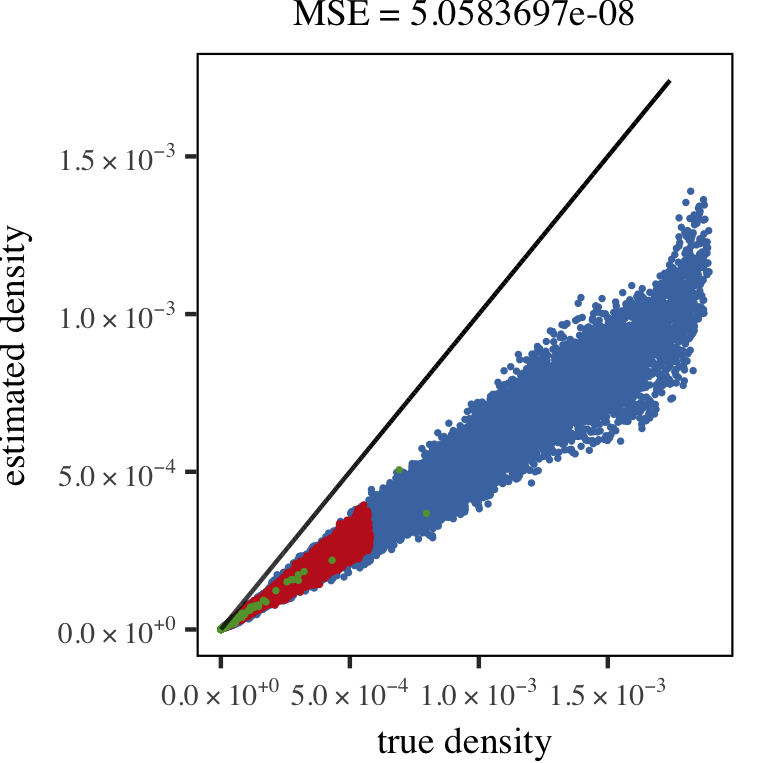
\includegraphics[keepaspectratio=true, width=\textwidth, height=0.23\textheight]{result/img/results_ferdosi_2_60000_mbe_silverman}
	\caption{Set \ferdosiTwo, \mbe}
	\label{fig:results:multisphere:mbe:ferdosi2}
\end{subfigure}
% Baakman 2, MBE
\begin{subfigure}{0.23\textwidth}
	\centering
	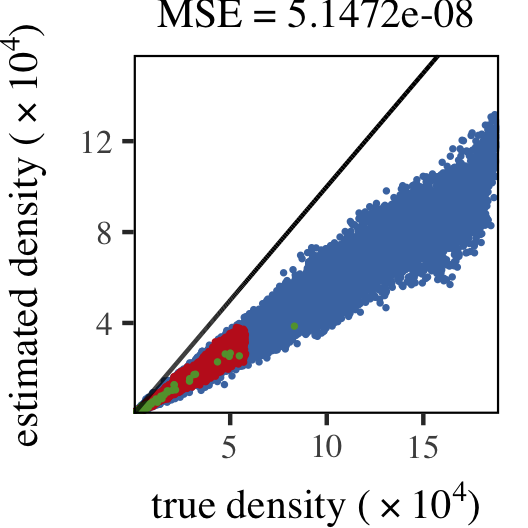
\includegraphics[keepaspectratio=true, width=\textwidth, height=0.23\textheight]{result/img/results_baakman_2_60000_mbe_silverman}
	\caption{Set \baakmanTwo, \mbe}
	\label{fig:results:multisphere:mbe:baakman2}
\end{subfigure}
% Ferdosi 2, SAMBE
\begin{subfigure}{0.23\textwidth}
	\centering
	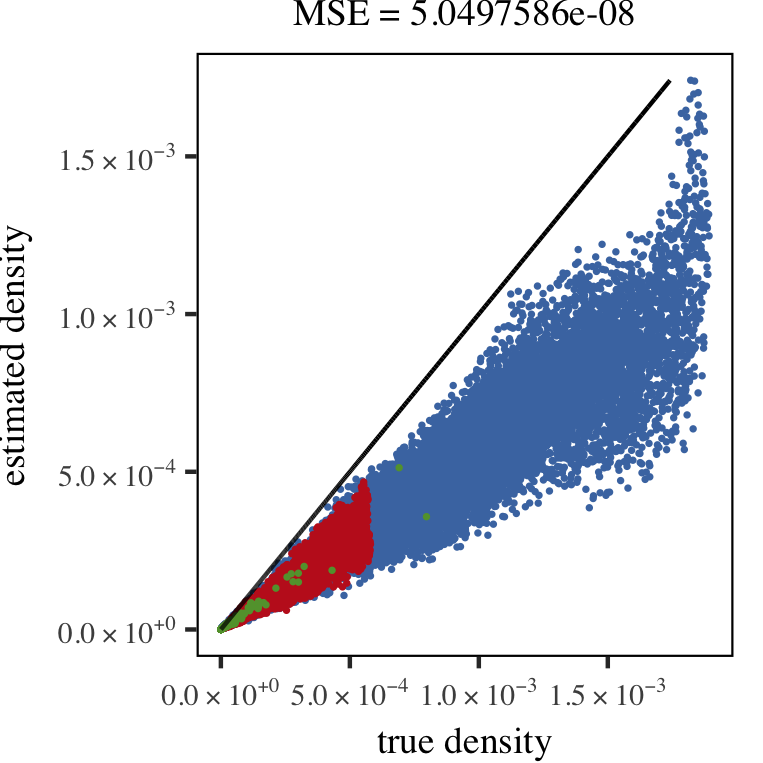
\includegraphics[keepaspectratio=true, width=\textwidth, height=0.23\textheight]{result/img/results_ferdosi_2_60000_sambe_silverman}
	\caption{Set \ferdosiTwo, \sambe}
	\label{fig:results:multisphere:sambe:ferdosi2}
\end{subfigure}
% Baakman 2, SAMBE
\begin{subfigure}{0.23\textwidth}
	\centering
	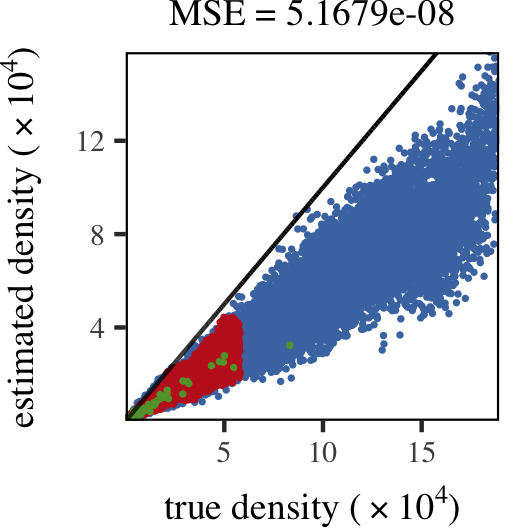
\includegraphics[keepaspectratio=true, width=\textwidth, height=0.23\textheight]{result/img/results_baakman_2_60000_sambe_silverman}
	\caption{Set \baakmanTwo, \sambe}
	\label{fig:results:multisphere:sambe:baakman2}
\end{subfigure}
	\caption{Plots of the true versus estimated density of datasets \ferdosiTwo and \baakmanTwo for the shape-adaptive and the symmetric Modified Breiman Estimator.}
	\label{fig:results:multiSphere:two:comparativePlots}
\end{figure}

\begin{figure}
	\centering
	%!TEX root = ../../paper.tex

% Ferdosi 3, MBE
\begin{subfigure}{0.33\textwidth}
	\centering
	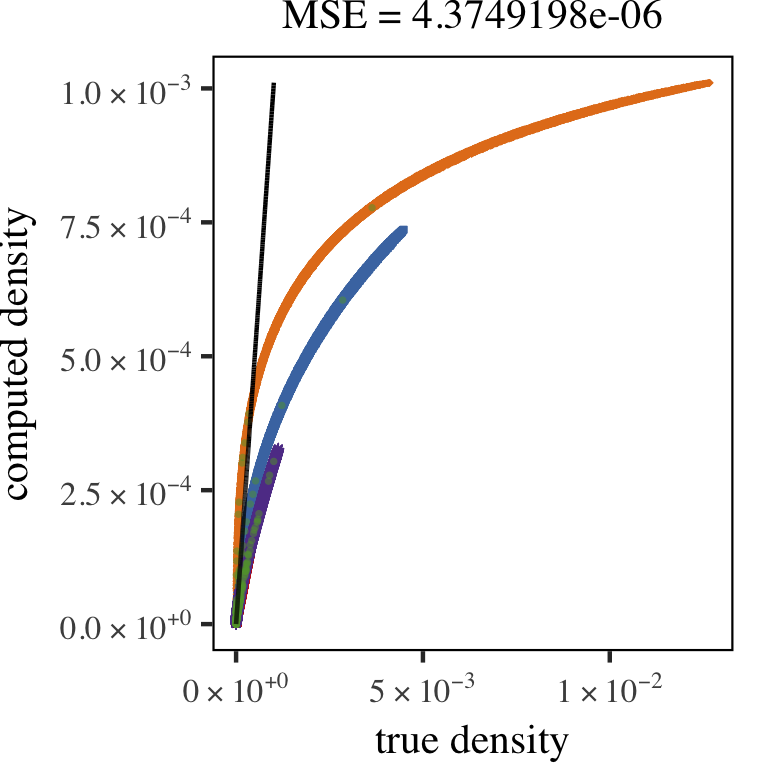
\includegraphics[keepaspectratio=true, width=\textwidth, height=0.23\textheight]{result/img/results_ferdosi_3_120000_mbe_silverman.png}
	\caption{Set \ferdosiThree, \mbe}
	\label{fig:results:multisphere:mbe:ferdosi3}
\end{subfigure}
% Baakman 3, MBE
\begin{subfigure}{0.33\textwidth}
	\centering
	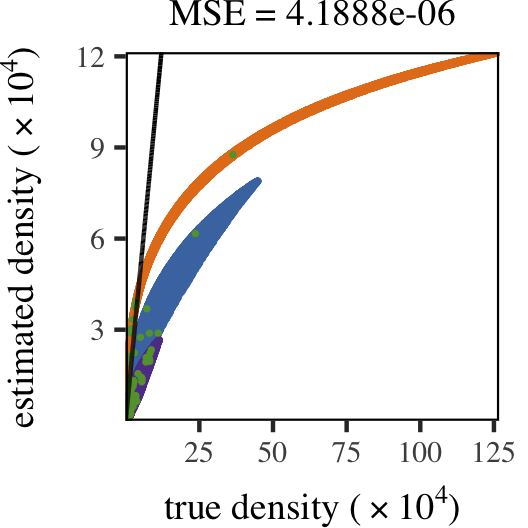
\includegraphics[keepaspectratio=true, width=\textwidth, height=0.23\textheight]{result/img/results_baakman_3_120000_mbe_silverman}
	\caption{Set \baakmanThree, \mbe}
	\label{fig:results:multisphere:mbe:baakman3}
\end{subfigure}	
% Ferdosi 3, SAMBE
\begin{subfigure}{0.33\textwidth}
	\centering
	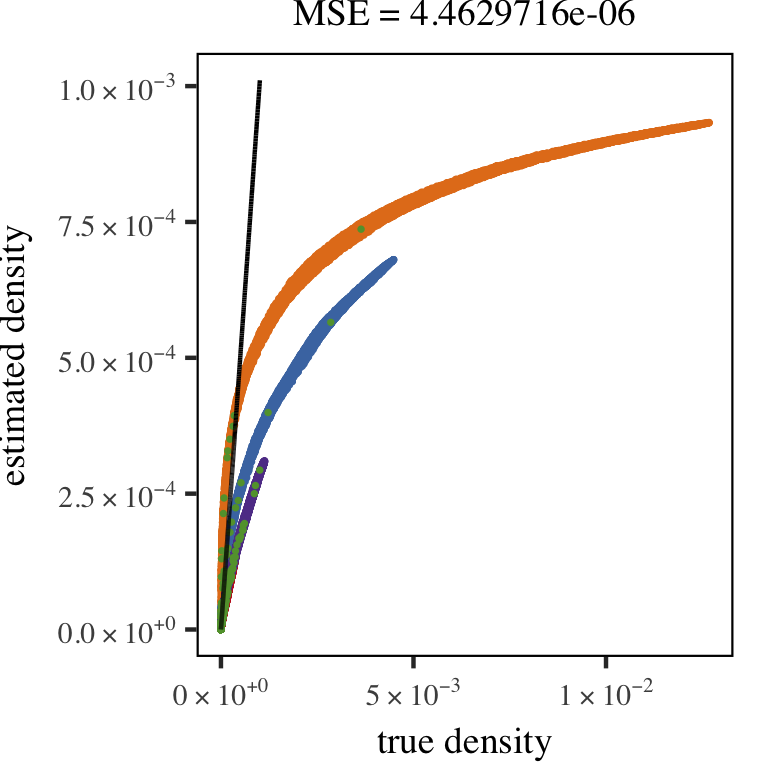
\includegraphics[keepaspectratio=true, width=\textwidth, height=0.23\textheight]{result/img/results_ferdosi_3_120000_sambe_silverman}
	\caption{Set \ferdosiThree, \sambe}
	\label{fig:results:multisphere:sambe:ferdosi3}
\end{subfigure}
% Baakman 3, SAMBE
\begin{subfigure}{0.33\textwidth}
	\centering
	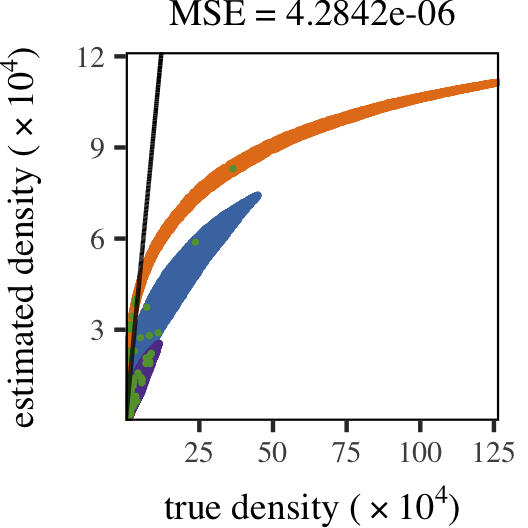
\includegraphics[keepaspectratio=true, width=\textwidth, height=0.23\textheight]{result/img/results_baakman_3_120000_sambe_silverman}
	\caption{Set \baakmanThree, \sambe}
	\label{fig:results:multisphere:sambe:baakman3}
\end{subfigure}	
	\caption{The estimated density plotted as a function of the true density for datasets \ferdosiThree and \baakmanThree for \mbe and \sambe.}
	\label{fig:results:multiSphere:three:comparativePlots}
\end{figure}

\begin{table}
	\centering
	%!TEX root = ../../paper.tex

\begin{tabular}{l*{2}{S[scientific-notation=true, round-mode=places,round-precision=3]}}
\toprule
~ 				& \multicolumn{2}{c}{Estimator}\\ \cmidrule{2-3}
Set				& {\mbe}					& {\sambe}	\\
\midrule
\ferdosiOne		& 8.30580618349064E-09		&  8.9087329457441E-09 \\
\baakmanOne		& 1.49022877061299E-08		&  1.5398737157543E-08 \\	
\baakmanFour	& 2.93709420107411E-08		&  2.9634323205557E-08 \\	
\baakmanFive	& 5.57179476550916E-08		&  5.5847473903432E-08 \\	
\bottomrule
\end{tabular}
	\caption{Performance of the symmetric and the shape-adaptive Modified Breiman Estimator on the datasets containing multiple Gaussian distributions.} 	
	\label{tab:results:multiSphere:mse}
\end{table}

%Introduction
	In this section we present the results of the two estimators on dataset \ferdosiTwo, \baakmanTwo, \ferdosiThree, \baakmanThree.

% Ferdosi 2
	% General difference
	Comparing \cref{fig:results:multisphere:mbe:ferdosi2} with \cref{fig:results:multisphere:sambe:ferdosi2} we find that both estimators underestimate the density and that the densities estimated by the \sambe are spread out more than those estimated by \mbe. In spite of this the difference in \mse between the two estimators is small enough to be insignificant. 
	% Components
	The same holds for the \mse of the individual components.

% Baakman 2
	% General difference
	\Cref{fig:results:multisphere:mbe:baakman2,fig:results:multisphere:sambe:baakman2} show the same general trend as \cref{fig:results:multisphere:mbe:ferdosi2,fig:results:multisphere:sambe:ferdosi2}: both estimators underestimate, the shape-adaptive estimator less so than the symmetric estimator, but the differences between the two estimators are small. 
	% Components
	The differences in \MSE within the difference components between the estimators are negligible. 
	% Contrast to Ferdosi 2
	Comparing the performance of the estimators between datasets \ferdosiTwo and \baakmanTwo we find that the performance of both estimators hardly suffers from the elongation of the Gaussians. 

% Ferdosi 3
	% General Differnce

	% Components

% Baakman 3
	% General Differnce

	% Components

	% Constrast to Ferdosi 3


% General
	\todo[inline]{General observation?}
	\todo[inline]{What is the influence of the density of Gaussian?}